\section{Results}
After smaller-scale trials, DrawAFriend was released publicly on January 8th, 2013. In 88 days there were 14,270 drawings. There were three steps that were taken after the initial launch of DrawAFriend. First we collected drawings from six celebrities to create our initial correction vector field. Second we use the correction field to create an automatic stroke correction helper in the game. Lastly we evaluated the accuracy of our stroke correction helper by comparing the drawings created with and without it. 

\subsection{DrawAFriend Correction Vector Field}
In order to place the correction vector field into the game, we needed to prime it with some initial drawings. After four days the game had downloaded the game over 2000 times and created 6373 drawings. In total, players had already spent approximately 10 full 24 hour days drawing. We used these drawings to create the consensus came.

Players were given the option of drawing Facebook friends or one of an initial set of six celebrities: Robert Downey Jr., Angelina Jolie, Kim Kardashian, Barack Obama, Brad Pitt, or Kristen Stewart. From the drawings generated in the first four days, we manually chose 611 celebrity drawings to be used for analysis. Drawings that were chosen were ones where players had made an attempt to somewhat accurately draw the eyes. For this initial dataset this was about 10\%. The rest of the dataset had a large percentage of drawings where players had quickly drawn probably without zooming, and thus resembled a person like scribble. While the rest of the dataset could be used for analysis, we did not train our correction vector field on it.   The statistics in Figure \ref{fig:daf-stats} reference the 611 drawings.

\begin{figure}[b]
  \centering%
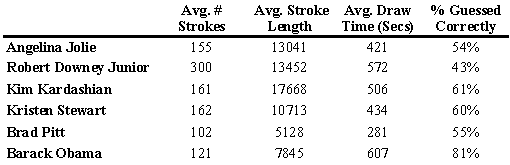
\includegraphics[height=1.1in]{./figures/daf-stats-cropped.pdf}
  \caption{Celebrity drawing statistics for 611 hand-picked drawings from the first four days after launch.}
  \label{fig:daf-stats}
\end{figure}

We ran our modified mean shift algorithm on this initial dataset to create the correction vector fields shown in Figure \ref{fig:image-table}. Our MATLAB implementation took under 5 minutes for each celebrity. The great majority of the time was spent in un-optimized nearest neighbor search.

\subsection {Drawing Enhancements}

We applied the correction vector field to interactively modify strokes during the drawing process in an enhanced, as yet unreleased, version of the game (see accompanying video). With no additional user interface elements to the existing DrawAFriend UI, we seamlessly add stroke auto-correction. As the user draws, strokes are subtly corrected at interactive rates on an iPhone 4. In general, the fact that corrections are being applied is almost invisible to the user. Instead, strokes appear where the user {\em intended} to draw.

%????Please see the \alex{Not sure how to reference the teaser on top} and the video for interactive examples.

We also applied the correction vector field retrospectively to improve the existing database of user drawings. The drawings are already quite good, making the corrections made by the vector field all the more impressive.  While the algorithm universally improves the images by making the celebrity far more recognizable, it does so without sacrificing style. For comparisons of the raw drawings and the corrected images please see Figure~\ref{fig:results} and our video and the supplementary files.

\subsection {Crowdsourced User Study}
In order to test the effectiveness of the stroke auto-correction, we instrumented the game to provide a large-scale user study. Every time a user drew one of the six celebrities (Robert Downey Jr., Angelina Jolie, Kim Kardashian, Barack Obama, Brad Pitt, or Kristen Stewart) they were unknowingly placed in one of two groups. One group drew the celebrities as before. The other group, unbeknownst to them, drew with the stroke auto-correction on. By comparing these two group, we can asses the effectiveness of the stroke auto-correction helper. By only adding a couple lines of code, we transformed a data collection crowd sourcing system into a large-scale user study.

\subsubsection {User Study Results}
500 players have "contributed" to the study which AB-tests the effect of our auto-correct on over 1300 drawings. Using this data we can assess recognition rates (measuring how good drawings are from the perspective of others). We also analyze undo rates (providing an insight into how artists like their own drawings). Finally we measure average "distance" from the artistic consensus (measuring how carefully artists are drawing). 

Our results show that universally autocorrect reduced undo rates (the ratio of undos to all other strokes). This effect is magnified for careful drawers (who undid 30\% or more strokes). Their undo rates decreased by a significant 5\% (Wilcoxian p-value = .045).  We view the drop in undo rates as an improvement in how players view their own drawings. Likewise we observe a significant change in the average distance to the consensus drawings. It increases by 18\% when our auto-corrector has turned on with a (p=1.65e-06), suggesting that artists do not need to draw as precisely. Interestingly, statistical analysis reveals that the auto-corrector does not significantly alter recognizability. We believe that our auto-corrector does not change players� drawing quality. Rather it makes reaching this level of quality easier by requiring less undos and less accuracy.

\begin{figure}
  \centering%
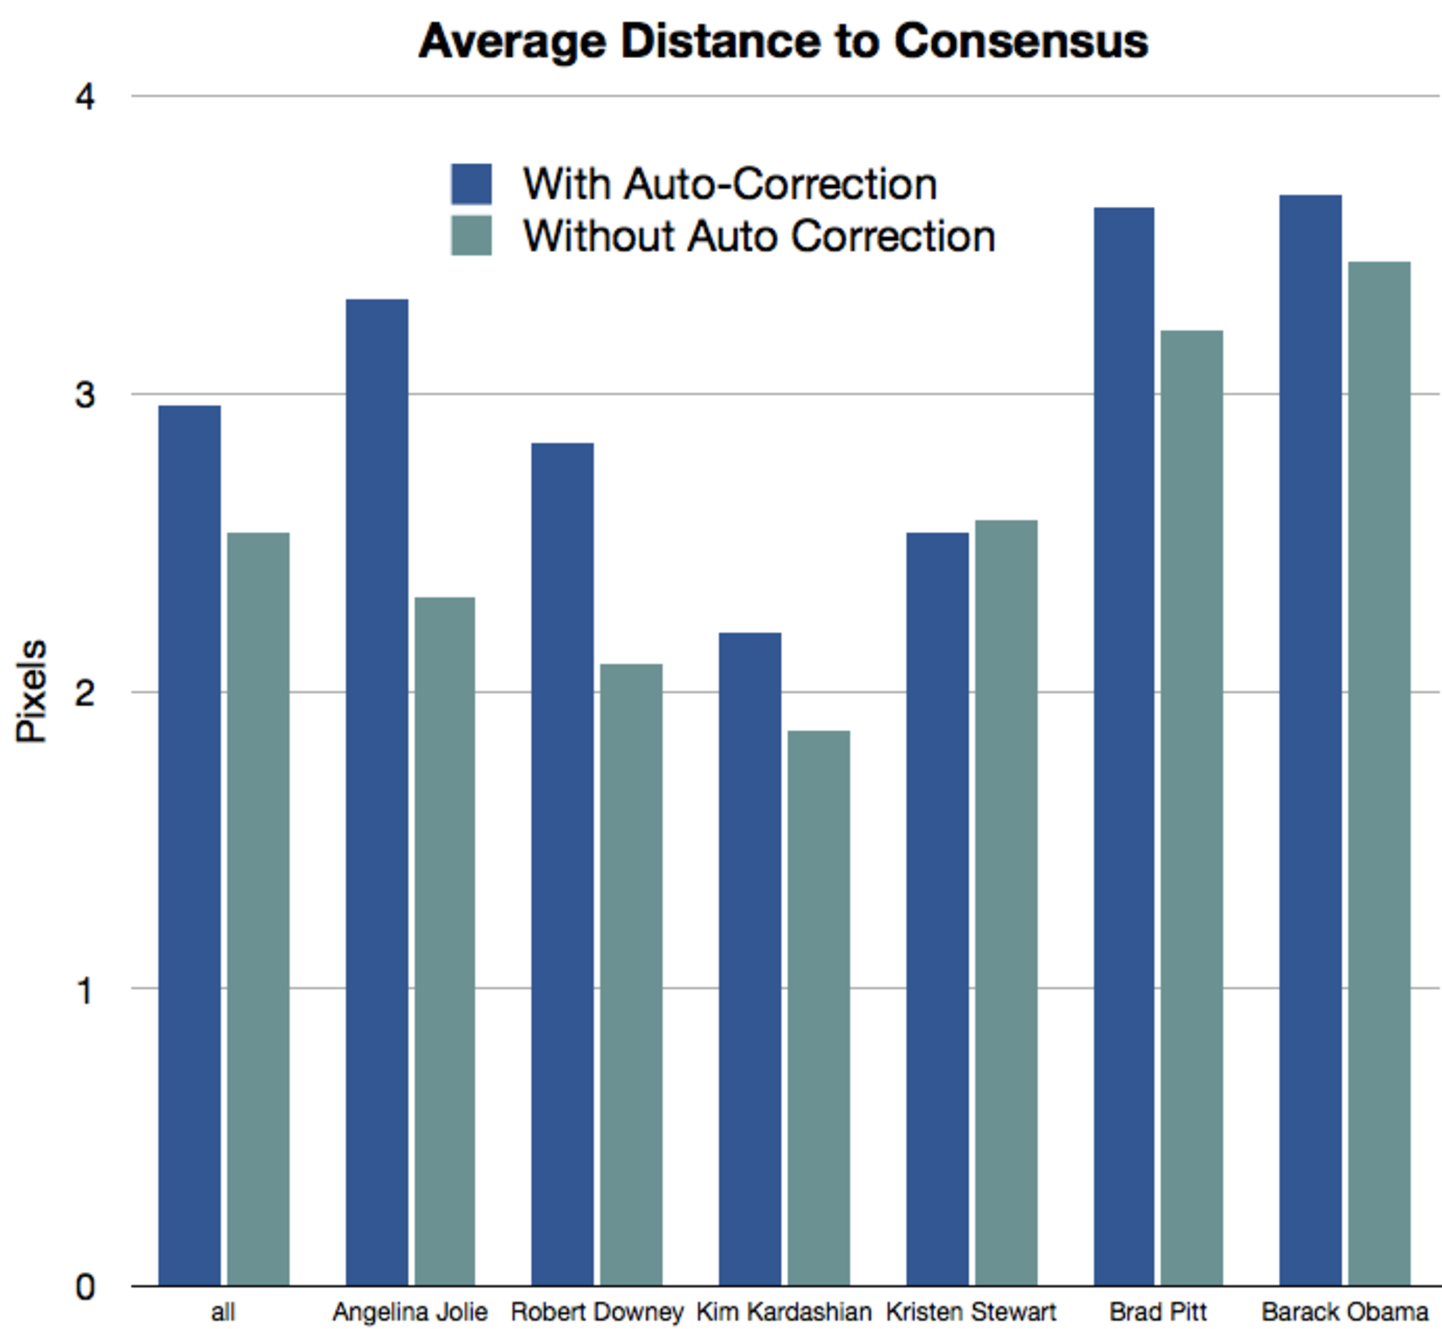
\includegraphics[width=3.5in]{./figures/userstudy/distanceToConsensus.pdf}
  \caption{The average distance to the consensus for each celebrity.}
  \label{fig:daf-distance}
\end{figure}

\begin{figure}
  \centering%
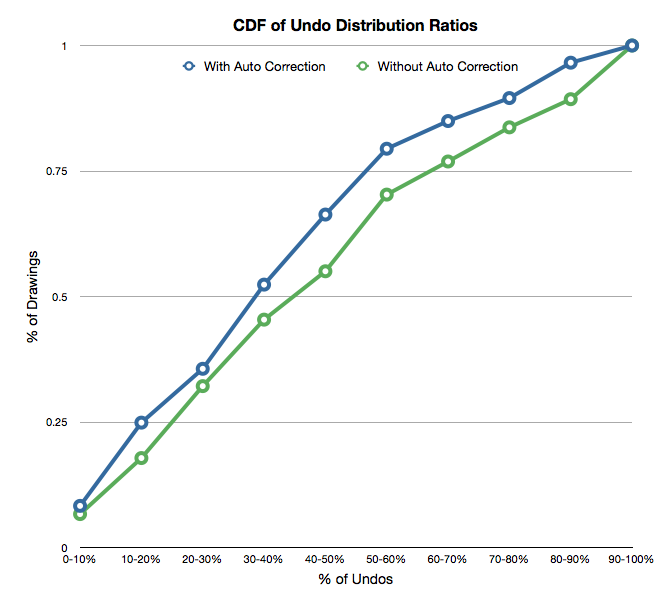
\includegraphics[width=3.5in]{./figures/userstudy/cdfUndos_chart.png}
  \caption{Temporary undo chart}
  \label{fig:daf-undo}
\end{figure}

\begin{figure}
  \centering%
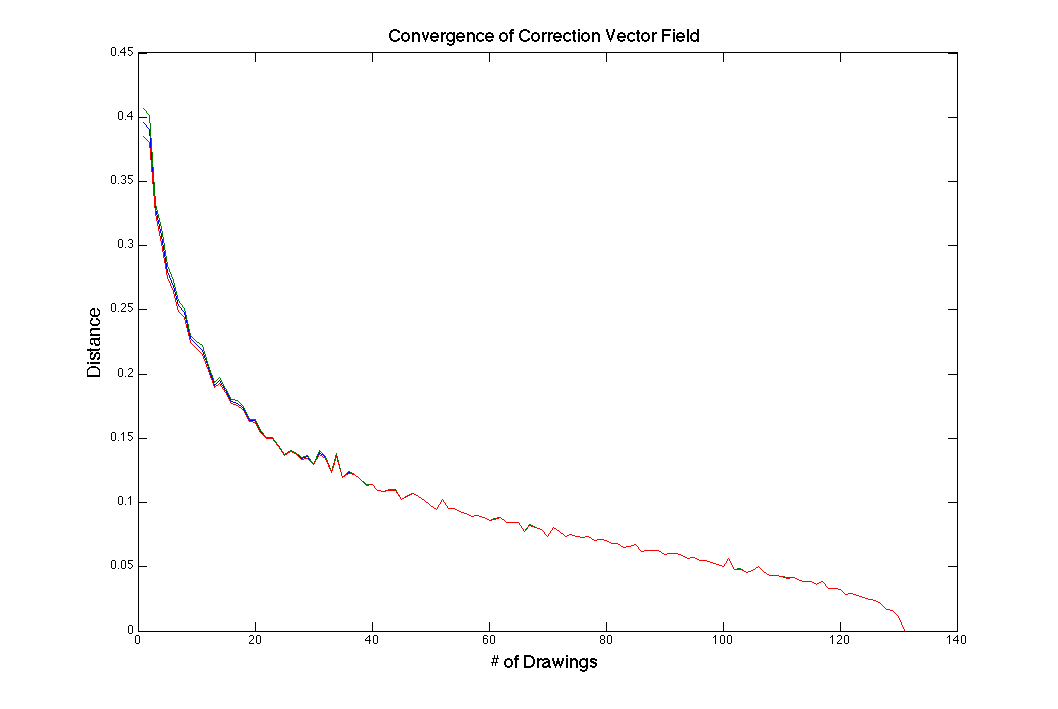
\includegraphics[width=3.5in]{./figures/userstudy/convergenceWithVar_131.png}
  \caption{Temporary Convergence Data, Trying to Smooth it out}
  \label{fig:daf-convergence}
\end{figure}



 

\begin{figure}
\centering
\begin{tabular}{ccccc}
\imgtbl{image_aj} & \imgtbl{avg_aj} & \imgtbl{dir_aj} & \imgtbl{mag_aj} & \imgtbl{edges_aj} \\
\imgtbl{image_bp} & \imgtbl{avg_bp} & \imgtbl{dir_bp} & \imgtbl{mag_bp} & \imgtbl{edges_bp} \\
\imgtbl{image_kk} & \imgtbl{avg_kk} & \imgtbl{dir_kk} & \imgtbl{mag_kk} & \imgtbl{edges_kk} \\
\imgtbl{image_ks} & \imgtbl{avg_ks} & \imgtbl{dir_ks} & \imgtbl{mag_ks} & \imgtbl{edges_ks} \\
\imgtbl{image_rd} & \imgtbl{avg_rd} & \imgtbl{dir_rd} & \imgtbl{mag_rd} & \imgtbl{edges_rd} \\
\imgtbl{image_bo} & \imgtbl{avg_bo} & \imgtbl{dir_bo} & \imgtbl{mag_bo} & \imgtbl{edges_bo} \\
(a) & (b) & (c) & (d) & (e)
\end{tabular}
\caption{DrawAFriend users draw one of six celebrities (a). We use our database of hundreds of drawings per subject -- shown averaged in (b) -- to precompute a \emph{correction vector field} (c) enabling real-time drawing assistance on the iPhone. The magnitude of our vector field (d) reveals a consensus of artistic renderings strikingly different than what we could compute with automated methods, such as a canny edge detector (e).}
\label{fig:image-table}
\end{figure}

\begin{figure*}[!t]
  \centering%
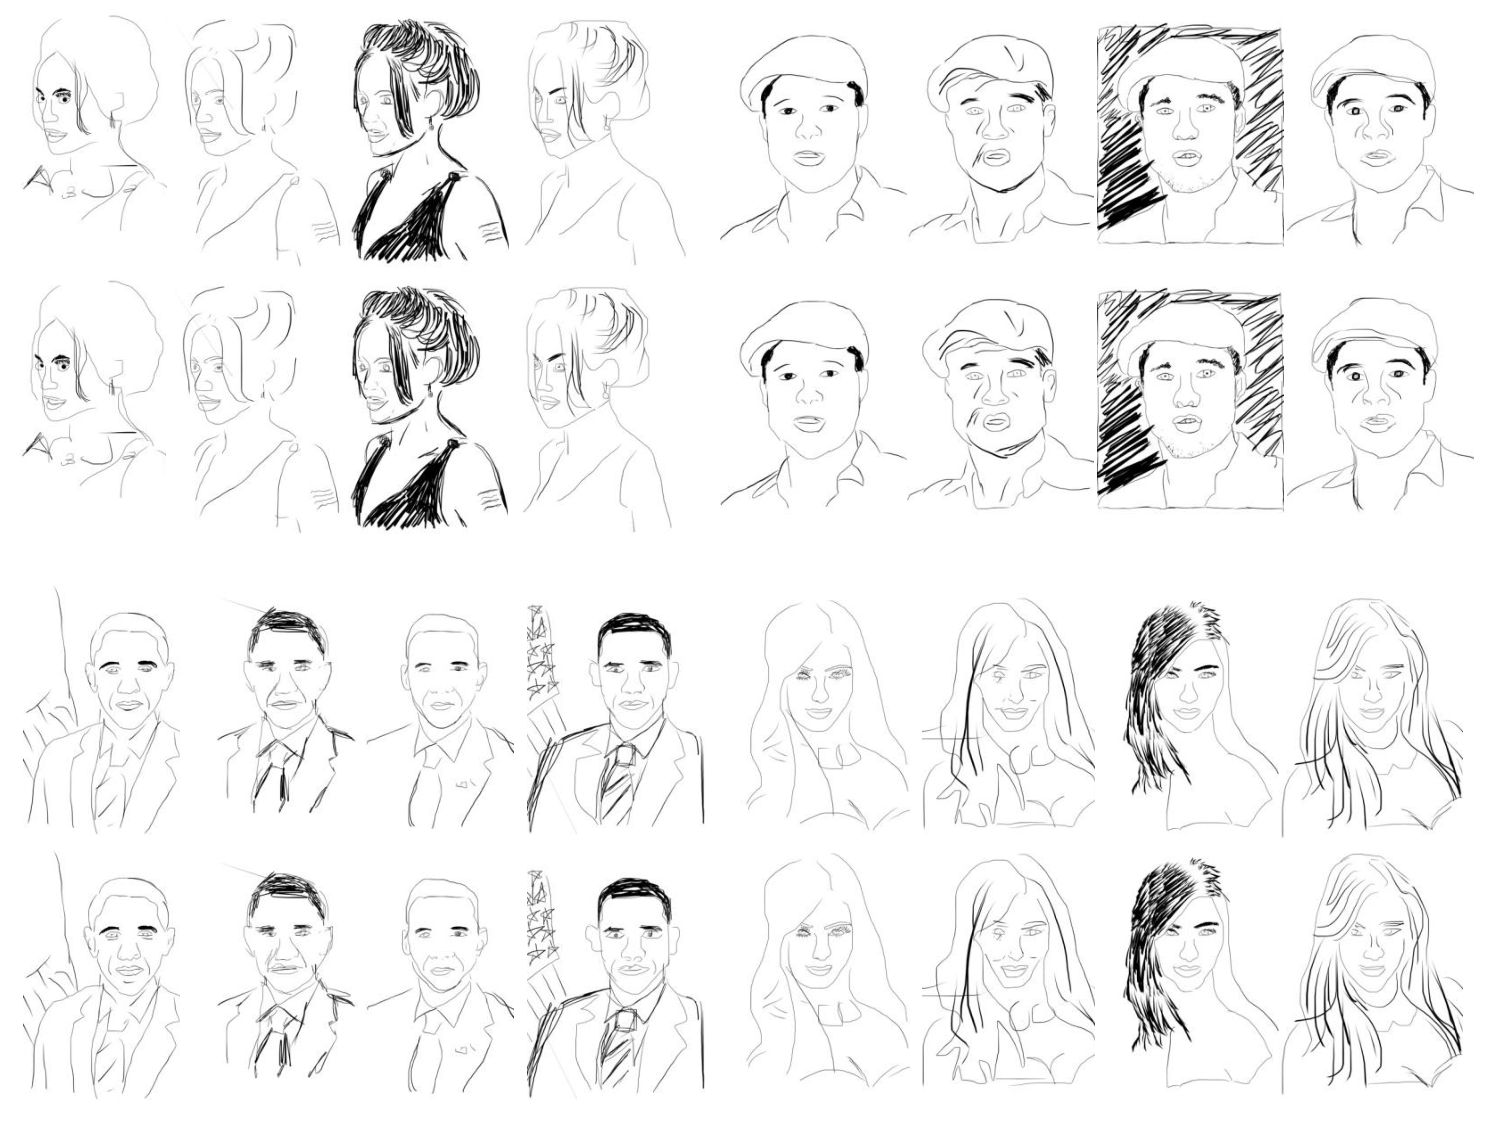
\includegraphics[width=7in]{./figures/ResultsAll.pdf}
\vspace{-0.35in}
  \caption{Celebrity drawings: original strokes (bottom rows) and after automatic adjustment to consensus (top rows). (Please see the supplementary files for more examples and also for an interface so you can flip between them.)}
\vspace{-0.25in}
  \label{fig:results}
\end{figure*}